
    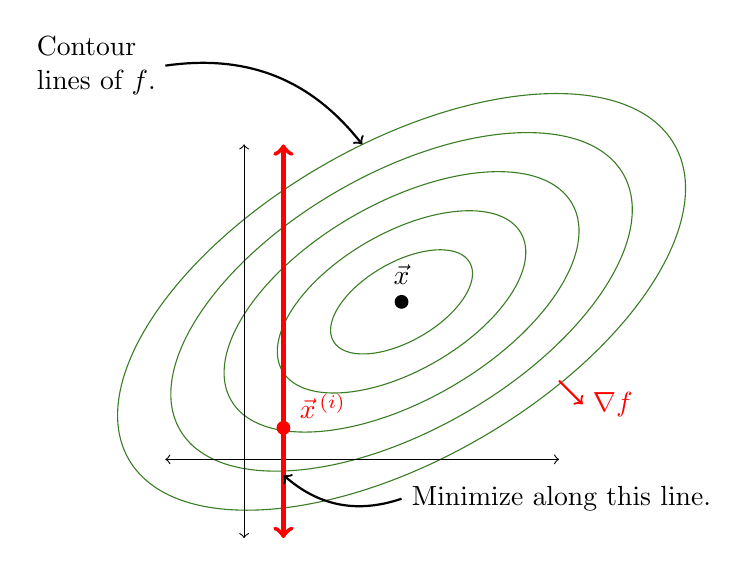
\begin{tikzpicture}
        \foreach \size in {1, 1.75, ..., 4} {
            \draw[OliveGreen, scale=\size, rotate=30] (0,0) ellipse (1cm and .5cm);
        };
        \node[circle, inner sep=0, minimum size=5pt,fill, label={$\vec{x}$}]() at (0,0){};

        \draw[<->] (-2, -3) -- (-2, 2);
        \draw[<->] (-3, -2) -- (2, -2);

        \node[ red, circle, inner sep=0, minimum size=5pt, fill,
        label={[red, xshift=5mm, yshift=-1mm]$\vec{x}^{\,(i)}$}
        ] () at (-1.5, -1.6){};

        \draw[<->, red, ultra thick] (-1.5, -3) -- (-1.5, 2);

        \draw[<-, thick] (-1.5, -2.2) to[bend right=30] (0, -2.5) node[right] () {Minimize along this line.};

        \draw[<-, thick] (-.5, 2) to[bend right=30] (-3, 3) node[left, xshift=5mm, text width=2cm] () {Contour lines of $f$.};

        \draw[->, thick, red] (2, -1) -- (2.3, -1.3) node[right](){$\nabla f$};
    \end{tikzpicture}
